\documentclass[a4paper, 11pt]{report}
\setcounter{tocdepth}{3}
\usepackage[utf8]{inputenc}
\usepackage[french]{babel}
\usepackage[T1]{fontenc}
\usepackage{graphicx}
\usepackage{xcolor}
\usepackage{booktabs}
\usepackage{tabularx}
\usepackage{fourier} 
\usepackage{array}
\usepackage{makecell}
\usepackage[top=2.5cm,bottom=2.5cm,right=2.5cm,left=2.5cm]{geometry}
\usepackage{amsmath}
\usepackage{xcolor}
\usepackage{colortbl,hhline}
\usepackage{subfig}
\usepackage{multirow}
\usepackage{comment}
\usepackage{makecell}
 \usepackage{fancyhdr}
 \pagestyle{fancy}

% \fancyhead[L]{\textsc{Gain d'information} }

\usepackage{algorithmic,algorithm}

\renewcommand{\listalgorithmname}{Liste des \ALG@name s}

\definecolor{yacine}{RGB}{241,241,241}
\usepackage{tikz}
\def\checkmark{\tikz\fill[scale=0.4](0,.35) -- (.25,0) -- (1,.7) -- (.25,.15) -- cycle;} 

\usepackage[backend=bibtex,style=numeric,sorting=nty]{biblatex}
\nocite{*} %Ausgabe aller Bibliographieeinträges
\usepackage{hyperref}
\hypersetup{
    linktoc=all,     %set to all if you want both sections and subsections linked
}


\begin{document}



\begin{figure}
\begin{center}

\includegraphics[scale=3]{critere2}
\end{center}
\end{figure}



 Préparé par : \\
 Mohammed Yacine BOUHEDADJA


\noindent \begin{center}
A rendre le mercredi 21/03/2018
\end{center}

\newpage
\tableofcontents

\chapter{Indice de GINI}

\section{Definition}
Le coefficient de Gini est une mesure statistique, mis au point afin de calculer le degré d'inégalité au sein d'une société (Salaire, niveau de vie, ...). Sa valeur varie entre 0 et 1, il est égal à 0 dans une situation d'égalité parfaite entre les individu de l'ensemble, et est égal à 1 dans dans la situation la plus inégalitaire possible.\\
Ce critère est utilisé dans la classification binaire, par l'algorithme \emph{CART} (\textsc{Classification And Regression Decision Tree)}, de façon a calculer l'indice de Gini de tous les testes, et d'en choisir celui ayant la valeur la plus basse.

\section{Formule}
\begin{center}
\begin{tabular}{| c |}
\hline
$Gini(S) = 1-\sum\limits_{j=0}^n 1- P_j^2$\\
\hline
\end{tabular}
\end{center}
Ou $P_j$ représente la fréquence relative à la classe j dans l'ensemble D


\section{Exemple}
Soit l'ensemble de donné suivant :\\

\begin{figure}[!h]
\begin{center}

\caption{Ensemble de données de départ}
\begin{tabular}{| l | l | l | l | l |}
\hline
\rowcolor{gray!25}
Temps & Température & Humidité & Vent & Jouer \\
\hline
Ensoleillé & Haute & Haute & Faux & \cellcolor{green}Non \\
\hline
Ensoleillé & Haute & Haute & Vrai & \cellcolor{green}Non \\
\hline
Couvert & Haute & Haute & Faux & \cellcolor{yellow}Oui \\
\hline
Pluvieux & Basse & Haute & Faux & \cellcolor{yellow}Oui \\
\hline
Pluvieux & Moyenne & Normal & Faux & \cellcolor{yellow}Oui \\
\hline
Pluvieux & Moyenne & Normal & Vrai &  \cellcolor{green}Non \\
\hline
Couvert & Moyenne & Normal & Vrai &  \cellcolor{yellow}Oui \\
\hline
Ensoleillé & Basse & Haute & Faux &  \cellcolor{green}Non \\
\hline
Ensoleillé & Moyenne & Normal & Faux &  \cellcolor{yellow}Oui \\
\hline
Pluvieux & Basse & Normal & Faux &  \cellcolor{yellow}Oui \\
\hline
Ensoleillé & Basse & Normal & Vrai &  \cellcolor{yellow}Oui \\
\hline
Couvert & Basse & Haute & Vrai &  \cellcolor{yellow}Oui \\
\hline
Couvert & Haute & Normal & Faux &  \cellcolor{yellow}Oui \\
\hline
Pluvieux & Moyenne & Haute & Vrai &  \cellcolor{green}Non \\
\hline
\end{tabular}
\end{center}

\end{figure}

\begin{itemize}

\item Recherche du teste de division

\begin{enumerate}

\item Temps\\
$Gini(Temps = ensoleillé) = 1 - ((\frac{2}{5})^2 + (\frac{3}{5})^2)=0.48 $
\\$Gini(Temps = pluvieux) = 1 - ((\frac{3}{5})^2 + (\frac{2}{5})^2)=0.48 $
\\$Gini(Temps = couvert) = 1 - ((\frac{5}{5})^2 =0 $

\item Température\\
$Gini(Temperature = haute) = 1 - ((\frac{2}{4})^2 + (\frac{2}{4})^2)=0.5 $
\\$Gini(Temperature = basse) = 1 - ((\frac{4}{5})^2 + (\frac{1}{5})^2)=0.32 $
\\$Gini(Temperature = moyenne) = 1 - ((\frac{3}{5})^2 + (\frac{2}{5})^2)=0.39 $

\item Humidité\\
$Gini(Humidité = haute) = 1 - ((\frac{2}{7})^2 + (\frac{5}{7})^2)=0.408 $
\\$Gini(Humidité = normal) = 1 - ((\frac{3}{7})^2 + (\frac{4}{7})^2)=0.489 $

\item Vent\\
$Gini(Vent = vrai) = 1 - ((\frac{3}{6})^2 + (\frac{3}{6})^2)=0.5 $
\\$Gini(Vent = faux) = 1 - ((\frac{6}{8})^2 + (\frac{2}{8})^2)=0.378 $
\end{enumerate}
\end{itemize}
La division se fera par rapport au teste Temps = couvert 

\begin{figure}[!h]
\begin{center}
\caption{Temps = couvert}
\label{ens1}
\begin{tabular}{| l | l | l | l | l |}
\hline
\rowcolor{gray!25}
Temps & Température & Humidité & Vent & Jouer \\
Couvert & Haute & Haute & Faux & \cellcolor{yellow}Oui \\
\hline
Couvert & Moyenne & Normal & Vrai &  \cellcolor{yellow}Oui \\
\hline
Couvert & Basse & Haute & Vrai & \cellcolor{yellow}Oui \\
\hline
Couvert & Haute & Normal & Faux &  \cellcolor{yellow}Oui \\
\hline
\end{tabular}
\end{center}
Sous ensemble homogène par rapport à la variable de classe, arrêt.

\end{figure}





\begin{figure}[!h]
\caption{Temps != couvert}
\label{ens2}
\begin{center}
\begin{tabular}{| l | l | l | l | l |}
\hline
\rowcolor{gray!25}
Temps & Température & Humidité & Vent & Jouer \\
\hline
Ensoleillé & Haute & Haute & Faux & \cellcolor{green}Non \\
\hline
Ensoleillé & Haute & Haute & Vrai & \cellcolor{green}Non \\
\hline
Pluvieux & Basse & Haute & Faux & \cellcolor{yellow}Oui \\
\hline
Pluvieux & Moyenne & Normal & Faux & \cellcolor{yellow}Oui \\
\hline
Pluvieux & Moyenne & Normal & Vrai &  \cellcolor{green}Non \\
\hline
Ensoleillé & Basse & Haute & Faux &  \cellcolor{green}Non \\
\hline
Ensoleillé & Moyenne & Normal & Faux &  \cellcolor{yellow}Oui \\
\hline
Pluvieux & Basse & Normal & Faux &  \cellcolor{yellow}Oui \\
\hline
Ensoleillé & Basse & Normal & Vrai &  \cellcolor{yellow}Oui \\
\hline
Pluvieux & Moyenne & Haute & Vrai &  \cellcolor{green}Non \\
\hline
\end{tabular}
\end{center}
\end{figure}
Sous ensemble hétérogène par rapport a la variable de classe, continuer son développement.

Recherche de teste de division

\begin{enumerate}
\item Temps\\
$Gini(Temps = ensoleillé) = 1 - ((\frac{2}{5})^2 + (\frac{3}{5})^2)=0.48 $\\
$Gini(Temps = pluvieux) = 1 - ((\frac{3}{5})^2 + (\frac{2}{5})^2)=0.48 $\\
\item Température\\
$Gini(Temperature = haute) = 1 - ((\frac{2}{2})^2 + ( 0 )=0 $\\
$Gini(Temperature = basse) = 1 - ((\frac{3}{4})^2 + (\frac{1}{4})^2)=0.375 $\\
$Gini(Temperature = moyenne) = 1 - ((\frac{2}{4})^2 + (\frac{2}{4})^2)=0.5 $\\

\item Humidité\\
$Gini(Humidité = haute) = 1 - ((\frac{1}{5})^2 + (\frac{4}{5})^2)=0.32 $\\
$Gini(Humidité = normal) = 1 - ((\frac{4}{5})^2 + (\frac{1}{5})^2)=0.32 $\\

\item Vent\\
$Gini(Vent = faux) = 1 - ((\frac{4}{6})^2 + (\frac{2}{6})^2)=0.45 $\\
$Gini(Vent = vrai) = 1 - ((\frac{1}{4})^2 + (\frac{3}{4})^2)=0.375 $
\end{enumerate}
La division se fera par rapport au teste Température=haute

\begin{figure}[!h]
\caption{Température = haute}
\label{ens3}
\begin{center}
\begin{tabular}{| l | l | l | l | l |}
\hline
\rowcolor{gray!25}
Temps & Température & Humidité & Vent & Jouer \\
\hline
Ensoleillé & Haute & Haute & Faux & \cellcolor{green}Non \\
\hline
Ensoleillé & Haute & Haute & Vrai & \cellcolor{green}Non \\
\hline
\end{tabular}
\end{center}
Sous ensemble homogène par rapport à la variable de classe, arrêt.
\end{figure}
\begin{figure}[!h]
\caption{Température != haute}
\label{ens4}
\begin{center}
\begin{tabular}{| l | l | l | l | l |}
\hline
\rowcolor{gray!25}
Temps & Température & Humidité & Vent & Jouer \\
\hline
Pluvieux & Basse & Haute & Faux & \cellcolor{yellow}Oui \\
\hline
Pluvieux & Moyenne & Normal & Faux & \cellcolor{yellow}Oui \\
\hline
Pluvieux & Moyenne & Normal & Vrai &  \cellcolor{green}Non \\
\hline
Ensoleillé & Basse & Haute & Faux &  \cellcolor{green}Non \\
\hline
Ensoleillé & Moyenne & Normal & Faux &  \cellcolor{yellow}Oui \\
\hline
Pluvieux & Basse & Normal & Faux &  \cellcolor{yellow}Oui \\
\hline
Ensoleillé & Basse & Normal & Vrai &  \cellcolor{yellow}Oui \\
\hline
Pluvieux & Moyenne & Haute & Vrai &  \cellcolor{green}Non \\
\hline
\end{tabular}
\end{center}
Sous ensemble hétérogène par rapport a la variable de classe, continuer son développement.
\end{figure}

Recherche de teste de division


\begin{enumerate}
\item Temps\\
$Gini(Temps = ensoleillé) = 1 - ((\frac{1}{3})^2 + (\frac{2}{3})^2)=0.45 $\\
$Gini(Temps = pluvieux) = 1 - ((\frac{3}{5})^2 + (\frac{2}{5})^2)=0.48 $\\
\item Température\\
$Gini(Temperature = basse) = 1 - ((\frac{3}{4})^2 + (\frac{1}{4})^2)=0.375 $\\
$Gini(Temperature = moyenne) = 1 - ((\frac{2}{4})^2 + (\frac{2}{4})^2)=0.5 $\\

\item Humidité\\
$Gini(Humidité = haute) = 1 - ((\frac{1}{3})^2 + (\frac{2}{3})^2)=0.45 $\\
$Gini(Humidité = normal) = 1 - ((\frac{4}{5})^2 + (\frac{1}{5})^2)=0.32 $\\

\item Vent\\
$Gini(Vent = faux) = 1 - ((\frac{4}{5})^2 + (\frac{1}{5})^2)=0.32 $\\
$Gini(Vent = vrai) = 1 - ((\frac{1}{3})^2 + (\frac{2}{3})^2)=0.45 $
\end{enumerate}

La division se fera par rapport à un des testes suivant :  Température=haute, vent=faux. \\Nous allons le faire par rapport au premier (Humidité=normal).
\begin{figure}[!h]
\caption{Humidité = normal}
\label{ens5}
\begin{center}
\begin{tabular}{| l | l | l | l | l |}
\hline
\rowcolor{gray!25}
Temps & Température & Humidité & Vent & Jouer \\
\hline
Pluvieux & Moyenne & Normal & Faux & \cellcolor{yellow}Oui \\
\hline
Pluvieux & Moyenne & Normal & Vrai &  \cellcolor{green}Non \\
\hline
Ensoleillé & Moyenne & Normal & Faux &  \cellcolor{yellow}Oui \\
\hline
Pluvieux & Basse & Normal & Faux &  \cellcolor{yellow}Oui \\
\hline
Ensoleillé & Basse & Normal & Vrai &  \cellcolor{yellow}Oui \\
\hline
\end{tabular}
\end{center}
Sous ensemble (A) hétérogène par rapport a la variable de classe, continuer son développement.
\end{figure}

\begin{figure}[!h]
\caption{Humidité != normal}
\label{ens6}
\begin{center}
\begin{tabular}{| l | l | l | l | l |}
\hline
\rowcolor{gray!25}
Temps & Température & Humidité & Vent & Jouer \\
\hline
Pluvieux & Basse & Haute & Faux & \cellcolor{yellow}Oui \\
\hline
Ensoleillé & Basse & Haute & Faux &  \cellcolor{green}Non \\
\hline
Pluvieux & Moyenne & Haute & Vrai &  \cellcolor{green}Non \\
\hline
\end{tabular}
\end{center}
Sous ensemble (B) hétérogène par rapport a la variable de classe, continuer son développement.
\end{figure}

\begin{enumerate}
\item Sous ensemble A\\
Recherche de teste de division



\begin{enumerate}
\item Temps\\
$Gini(Temps = ensoleillé) = 1 - ((\frac{1}{3})^2 + (\frac{2}{3})^2)=0.45 $\\
$Gini(Temps = pluvieux) = 1 - ((\frac{2}{2})^2 + ( 0 )=0 $\\
\item Température\\
$Gini(Temperature = basse) = 1 - ((\frac{2}{2})^2 + ( 0 )=0 $\\
$Gini(Temperature = moyenne) = 1 - ((\frac{2}{3})^2 + (\frac{1}{3})^2)=0.45 $\\

\item Vent\\
$Gini(Vent = faux) = 1 - ((\frac{3}{3})^2 + ( 0 )=0 $\\
$Gini(Vent = vrai) = 1 - ((\frac{1}{2})^2 + (\frac{1}{2})^2)=0.5 $
\end{enumerate}
La division se ferra par rapport à un des testes suivants : Temps=pluvieux ou Vent=faux, nous allons la faire par rapport au premier teste (Temps=pluvieux).


\begin{figure}[!h]
\caption{Temps != pluvieux}
\label{ens8}
\begin{center}
\begin{tabular}{| l | l | l | l | l |}
\hline
\rowcolor{gray!25}
Temps & Température & Humidité & Vent & Jouer \\
\hline
Ensoleillé & Moyenne & Normal & Faux &  \cellcolor{yellow}Oui \\
\hline
Ensoleillé & Basse & Normal & Vrai &  \cellcolor{yellow}Oui \\
\hline
\end{tabular}
\end{center}
Sous ensemble homogène par rapport a la variable de classe, arrêt.
\end{figure}

\begin{figure}[!h]
\caption{Temps = pluvieux}
\label{ens7}
\begin{center}
\begin{tabular}{| l | l | l | l | l |}
\hline
\rowcolor{gray!25}
Temps & Température & Humidité & Vent & Jouer \\
\hline
Pluvieux & Moyenne & Normal & Faux & \cellcolor{yellow}Oui \\
\hline
Pluvieux & Moyenne & Normal & Vrai &  \cellcolor{green}Non \\
\hline
Pluvieux & Basse & Normal & Faux &  \cellcolor{yellow}Oui \\
\hline
\end{tabular}
\end{center}
Sous ensemble hétérogène par rapport a la variable de classe, continuer son développement.
\end{figure}

%%%%%%%%%%%%%%%%%%%%%%%%%%%%%%%%%%%%%%%%%%%%%%%%
%%%%%%%%%%%%%%%%%%%%%%%%%%%%%%%%%%%%%%%%%%%%%%%%
%%%%%%%%%%%%%%%%%%%%%%%%%%%%%%%%%%%%%%%%%%%%%%%%

Recherche de teste de division

\begin{enumerate}
\item Température\\
$Gini(Temperature = basse) = 1 - ((\frac{1}{1})^2 + ( 0 )=0 $\\
$Gini(Temperature = moyenne) = 1 - ((\frac{1}{2})^2 + (\frac{1}{2})^2)=0.5 $\\

\item Vent\\
$Gini(Vent = faux) = 1 - ((\frac{2}{2})^2 + ( 0 )=0 $\\
$Gini(Vent = vrai) = 1 - ((\frac{1}{1})^2 + ( 0 )=0 $
\end{enumerate}
Division par rapport au teste Vent = vrai

\begin{figure}[!h]
\caption{Vent = vrai}
\label{ens9}
\begin{center}
\begin{tabular}{| l | l | l | l | l |}
\hline
\rowcolor{gray!25}
Temps & Température & Humidité & Vent & Jouer \\
\hline
Pluvieux & Moyenne & Normal & Vrai &  \cellcolor{green}Non \\
\hline
\end{tabular}
\end{center}
\end{figure}
Sous ensemble homogène par rapport à la variable de classe, arrêt.
\begin{figure}[!h]
\caption{Vent != Vrai}
\label{ens10}
\begin{center}
\begin{tabular}{| l | l | l | l | l |}
\hline
\rowcolor{gray!25}
Temps & Température & Humidité & Vent & Jouer \\
\hline
Pluvieux & Moyenne & Normal & Faux & \cellcolor{yellow}Oui \\
\hline
Pluvieux & Basse & Normal & Faux &  \cellcolor{yellow}Oui \\
\hline
\end{tabular}
\end{center}
\end{figure}
Sous ensemble homogène par rapport à la variable de classe, arrêt.

\item Sous ensemble B\\
Recherche de teste de division


\begin{enumerate}
\item Temps\\
$Gini(Temps = ensoleillé) = 1 - ( ( 0 ) + (\frac{1}{1})^2 =0 $\\
$Gini(Temps = pluvieux) = 1 - ((\frac{1}{2})^2 + (\frac{1}{2})^2)=0.5 $\\
\item Température\\
$Gini(Temperature = basse) = 1 - ((\frac{1}{2})^2 + (\frac{1}{2})^2)=0.5 $\\
$Gini(Temperature = moyenne) = 1 - ( 0 ) + (\frac{1}{1})^2)=0 $\\

\item Vent\\
$Gini(Vent = faux) = 1 - ((\frac{1}{2})^2 + (\frac{1}{2})^2)=0.5 $\\
$Gini(Vent = vrai) = 1 - ( 0 )^2 + (\frac{1}{1})^2)=0 $
\end{enumerate}
Division par rapport au teste Temps=ensoleillé

\begin{figure}[!h]
\caption{Temps = ensoleillé}
\label{ens11}
\begin{center}
\begin{tabular}{| l | l | l | l | l |}
\hline
\rowcolor{gray!25}
Temps & Température & Humidité & Vent & Jouer \\
\hline
Ensoleillé & Basse & Haute & Faux &  \cellcolor{green}Non \\
\hline
\end{tabular}
\end{center}
\end{figure}
Sous ensemble homogène par rapport à la variable de classe, arrêt.

\begin{figure}[!h]
\caption{Temps != ensoleillé}
\label{ens12}
\begin{center}
\begin{tabular}{| l | l | l | l | l |}
\hline
\rowcolor{gray!25}
Temps & Température & Humidité & Vent & Jouer \\
\hline
Pluvieux & Basse & Haute & Faux & \cellcolor{yellow}Oui \\
\hline
Pluvieux & Moyenne & Haute & Vrai &  \cellcolor{green}Non \\
\hline
\end{tabular}
\end{center}
Sous ensemble hétérogène par rapport à la variable de classe, continuer son développement.
\end{figure}
Recherche de teste de division 

\begin{enumerate}
\item Température\\
$Gini(Temperature = basse) = 1 - ((\frac{1}{1})^2 + ( 0 ))=0 $\\
$Gini(Temperature = moyenne) = 1 - ( 0 ) + (\frac{1}{1})^2)=0 $\\

\item Vent\\
$Gini(Vent = faux) = 1 - ((\frac{1}{2})^2 + ( 0 )=0 $\\
$Gini(Vent = vrai) = 1 - ( 0 )^2 + (\frac{1}{1})^2)=0 $
\end{enumerate}
Division par rapport au teste Température=basse

\begin{figure}[!h]
\caption{Température = basse}
\label{ens12}
\begin{center}
\begin{tabular}{| l | l | l | l | l |}
\hline
\rowcolor{gray!25}
Temps & Température & Humidité & Vent & Jouer \\
\hline
Pluvieux & Basse & Haute & Faux & \cellcolor{yellow}Oui \\
\hline
\end{tabular}
\end{center}
Sous ensemble homogène par rapport à l'attribut de classe, arrêt
\end{figure}
\begin{figure}[!h]
\caption{Température != basse}
\label{ens12}
\begin{center}
\begin{tabular}{| l | l | l | l | l |}
\hline
\rowcolor{gray!25}
Temps & Température & Humidité & Vent & Jouer \\
\hline
Pluvieux & Moyenne & Haute & Vrai &  \cellcolor{green}Non \\
\hline
\end{tabular}
\end{center}
Sous ensemble homogène par rapport à l'attribut de classe, arrêt
\end{figure}



\end{enumerate}

TOUS LES SOUS ENSEMBLE SONS HOMOGÈNES : CRITÈRE D'ARRÊT ATTEINT.

\newpage
\section{L'arbre de décision}

\begin{figure}[!h]
\begin{center}
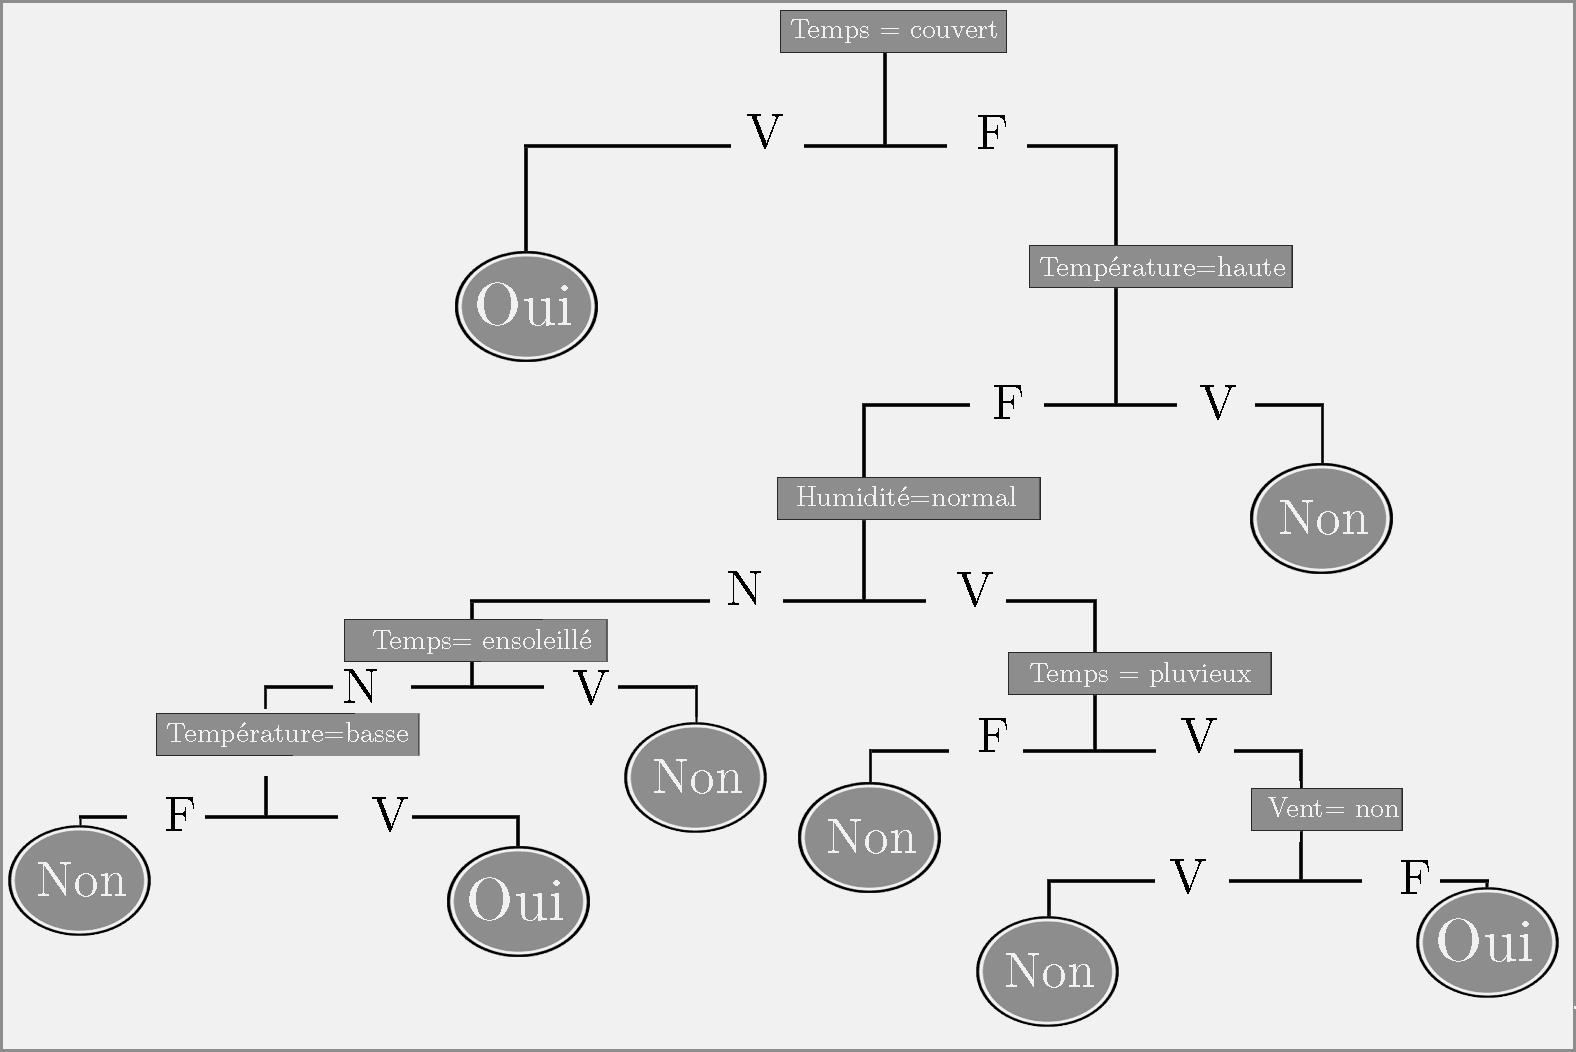
\includegraphics[scale=2]{figure_gini}
\end{center}
\caption{Arbre de décision binaire crée avec CART en utilisant l'indice de Gini}
\end{figure}



\chapter{Gain d'information}

\section{Definition}
Le gain d'information est un critère basé sur l'impureté, il utilise la mesure d'entropie comme mesure d'impureté ( mesure mise au point par Quinlan en 1987). Ce critère de division est utilisé par l'algorithme \textsc{Id3}.

\section{Formule}
Le Gain d'information d'un attribut T est égal a la différence entre l'entropie pré-division (nœud père p), et l'entropie post-division (par rapport à l'attribut T).
\begin{center}
\begin{tabular}{| c |}
\hline
$Gain(p,T) = Entropie(P) - \sum_{j=1}^n (P_j * Log_2(P_j)) $\\
% 1-\sum\limits_{j=0}^n 1- P_j^2$\\
\hline
\end{tabular}
\end{center}

\section{Exemple}
Soit l'ensemble de donné suivant :\\

\begin{figure}[!h]
\begin{center}

\caption{Ensemble de données de départ}
\begin{tabular}{| l | l | l | l | l |}
\hline
\rowcolor{gray!25}
Temps & Température & Humidité & Vent & Jouer \\
\hline
Ensoleillé & Haute & Haute & Faux & \cellcolor{green}Non \\
\hline
Ensoleillé & Haute & Haute & Vrai & \cellcolor{green}Non \\
\hline
Couvert & Haute & Haute & Faux & \cellcolor{yellow}Oui \\
\hline
Pluvieux & Basse & Haute & Faux & \cellcolor{yellow}Oui \\
\hline
Pluvieux & Moyenne & Normal & Faux & \cellcolor{yellow}Oui \\
\hline
Pluvieux & Moyenne & Normal & Vrai &  \cellcolor{green}Non \\
\hline
Couvert & Moyenne & Normal & Vrai &  \cellcolor{yellow}Oui \\
\hline
Ensoleillé & Basse & Haute & Faux &  \cellcolor{green}Non \\
\hline
Ensoleillé & Moyenne & Normal & Faux &  \cellcolor{yellow}Oui \\
\hline
Pluvieux & Basse & Normal & Faux &  \cellcolor{yellow}Oui \\
\hline
Ensoleillé & Basse & Normal & Vrai &  \cellcolor{yellow}Oui \\
\hline
Couvert & Basse & Haute & Vrai &  \cellcolor{yellow}Oui \\
\hline
Couvert & Haute & Normal & Faux &  \cellcolor{yellow}Oui \\
\hline
Pluvieux & Moyenne & Haute & Vrai &  \cellcolor{green}Non \\
\hline
\end{tabular}
\end{center}

\end{figure}

\begin{itemize}

\item Calcule de l'entropie de l'ensemble\\
Nous avons :\\
Nombre d'instance : 14

\[Nombre \ de \ classes \ : \ 2 \ \left\{ 
\begin{array}{l l}
  Oui : & \quad \text{ 9}\\
  Non : & \quad \text{ 5}\\ \end{array} \right. \]
$Entropie(P) = -((\frac{9}{14})Log_2(\frac{9}{14}) + (\frac{5}{14})Log_2(\frac{5}{14})) = 0.94$

\item Calcule de l'entropie de chacun des attributs
\begin{enumerate}
\item Temps 
\begin{table}[!h]
\begin{center}
\begin{tabular}{| l | c | c | c |}
\hline
 & Oui & Non & Nb d'instance\\
 \hline
Ensoleillé & 2 & 3 & 5 \\
\hline
Pluvieux & 3 & 2 & 5\\
\hline
Couvert & 4 & 0 & 4\\
\hline 
\end{tabular}
\caption{Table de comptage de l'attribut Temps}
\end{center}
\end{table}


$Entropie(Temps) = \frac{5}{14}(- (\frac{2}{5} Log_2(\frac{2}{5}) + \frac{3}{5} Log_2(\frac{3}{5}))) + \\
\frac{5}{14}(- (\frac{3}{5} Log_2(\frac{3}{5}) + \frac{2}{5} Log_2(\frac{2}{5}))) + \\
\frac{4}{14}(- \frac{4}{4} Log_2(\frac{4}{4}))\\
Entropie(Temps) = 0.69$
\item Température
\begin{table}[!h]
\begin{center}
\begin{tabular}{| l | c | c | c |}
\hline
 & Oui & Non & Nb d'instance\\
 \hline
Basse & 4 & 1 & 5 \\
\hline
Moyenne & 3 & 2 & 5\\
\hline
Haute & 2 & 2 & 4\\
\hline 
\end{tabular}
\caption{Table de comptage de l'attribut Température}
\end{center}
\end{table}

$Entropie(Température) = \frac{5}{14}(- (\frac{4}{5} Log_2(\frac{4}{5}) + \frac{1}{5} Log_2(\frac{1}{5}))) + \\
\frac{5}{14}(- (\frac{3}{5} Log_2(\frac{3}{5}) + \frac{2}{5} Log_2(\frac{2}{5}))) + \\
\frac{4}{14}(- (\frac{2}{4} Log_2(\frac{2}{4}) + \frac{2}{4} Log_2(\frac{2}{4})))\\
Entropie(Temps) = 0.89$

\item Humidité

\begin{table}[!h]
\begin{center}
\begin{tabular}{| l | c | c | c |}
\hline
 & Oui & Non & Nb d'instance\\
 \hline
Haute & 4 & 3 & 7 \\
\hline
Normal & 6 & 1 & 7\\
\hline 
\end{tabular}
\caption{Table de comptage de l'attribut Humidité}
\end{center}
\end{table}


$Entropie(Humidité) = \frac{7}{14}(- (\frac{4}{7} Log_2(\frac{4}{7}) + \frac{3}{7} Log_2(\frac{3}{7}))) + \\
\frac{7}{14}(- (\frac{6}{7} Log_2(\frac{6}{7}) + \frac{1}{7} Log_2(\frac{1}{7})))
Entropie(Temps) = 0.79$

\item Vent

\begin{table}[!h]
\begin{center}
\begin{tabular}{| l | c | c | c |}
\hline
 & Oui & Non & Nb d'instance\\
 \hline
Vrai & 3 & 3 & 6 \\
\hline
Faux & 6 & 2 & 8\\
\hline 
\end{tabular}
\caption{Table de comptage de l'attribut Vent}
\end{center}
\end{table}

$Entropie(Humidité) = \frac{6}{14}(- (\frac{3}{6} Log_2(\frac{3}{6}) + \frac{3}{6} Log_2(\frac{3}{6}))) + \\
\frac{8}{14}(- (\frac{6}{8} Log_2(\frac{6}{8}) + \frac{2}{8} Log_2(\frac{2}{8})))
Entropie(Temps) = 0.89$
\end{enumerate}

\newpage
\item Calcul du gain d'information de chaque attribut\\

\[ \thead{Gain(Temps) = 0.94 - 0.69 = 0.25 \\ 
Gain(Température) = 0.94 - 0.89 = 0.05 \\
Gain(Humidité) = 0.94 - 0.69 = 0.15\\
Gain(Vent) = 0.94 - 0.69 = 0.05
}\left\{ 
\begin{array}{l l}
 L'attribut choisi pour la division est : Temps & \quad \text{}\\
  \end{array} \right. \]

Étant donné que cet attribut se compose de trois valeurs, la division va générer trois sous ensemble, qui sont les suivant :\\

\begin{figure}[!h]
\begin{center}

\begin{tabular}{| l | l | l | l | l |}
\hline
\rowcolor{gray!25}
Temps & Température & Humidité & Vent & Jouer \\
\hline
Couvert & Haute & Haute & Faux & \cellcolor{yellow}Oui \\
\hline
Couvert & Moyenne & Normal & Vrai &  \cellcolor{yellow}Oui \\
\hline
Couvert & Basse & Haute & Vrai &  \cellcolor{yellow}Oui \\
\hline
Couvert & Haute & Normal & Faux &  \cellcolor{yellow}Oui \\
\hline
\end{tabular}
\end{center}
\caption{Sous ensemble A}
\end{figure}

\begin{table}[!h]
\begin{small}
\begin{tabular}{cc}

    \begin{minipage}{.5\linewidth}
   
\begin{tabular}{| l | l | l | l | l |}
\hline
Temps & Température & Humidité & Vent & Jouer \\
\hline
Ensoleillé & Haute & Haute & Faux & \cellcolor{green}Non \\
\hline
Ensoleillé & Haute & Haute & Vrai & \cellcolor{green}Non \\
Ensoleillé & Basse & Haute & Faux &  \cellcolor{green}Non \\
\hline
Ensoleillé & Moyenne & Normal & Faux &  \cellcolor{yellow}Oui \\
\hline
Ensoleillé & Basse & Normal & Vrai &  \cellcolor{yellow}Oui \\
\hline
\end{tabular}
      \caption{Sous ensemble C}

    \end{minipage} &

    \begin{minipage}{.5\linewidth}
\begin{tabular}{| l | l | l | l | l |}
\hline
Temps & Température & Humidité & Vent & Jouer \\
\hline
Pluvieux & Basse & Haute & Faux & \cellcolor{yellow}Oui \\
\hline
Pluvieux & Moyenne & Normal & Faux & \cellcolor{yellow}Oui \\
\hline
Pluvieux & Moyenne & Normal & Vrai &  \cellcolor{green}Non \\
\hline
Pluvieux & Basse & Normal & Faux &  \cellcolor{yellow}Oui \\
\hline
Pluvieux & Moyenne & Haute & Vrai &  \cellcolor{green}Non \\
\hline
\end{tabular} 
      \caption{Sous ensemble B}
 
    \end{minipage} 
\end{tabular}
\end{small}
\end{table}
Le sous ensemble A, correspondant a la valeur "Temps = couvert" est homogène, son développement s'arrête, 
contrairement au sous ensemble B et C.


\item Développement du sous ensemble B\\
\begin{itemize}
\item Calcul de l'entropie de l'ensemble 
$Entropie(P) = -((\frac{3}{5})Log_2(\frac{3}{5}) + (\frac{2}{5})Log_2(\frac{2}{5})) = 0.97$
\item Calcul de l'entropie de chaque attribut
\begin{enumerate}
\item Température 
$Entropie(Temperature) = \frac{2}{5}(- (\frac{1}{2} Log_2(\frac{1}{2}) + \frac{1}{2} Log_2(\frac{1}{2}))) + \\
\frac{1}{5}(- (\frac{1}{1} Log_2(\frac{1}{1}))) + \\
\frac{2}{4}(- (\frac{2}{2} Log_2(\frac{2}{2})))\\
Entropie(Temperature) = 0.4$
\item Humidité
$Entropie(Humidité) = \frac{3}{5}(- (\frac{3}{3} Log_2(\frac{3}{3})) + \\
\frac{2}{5}(- (\frac{2}{2} Log_2(\frac{2}{2}))\\
Entropie(Humidité) = 0$
\item Vent 
$Entropie(Vent) = \frac{3}{5}(- (\frac{1}{3} Log_2(\frac{1}{3}) + \frac{2}{3} Log_2(\frac{2}{3}))) + \\
\frac{2}{5}(- (\frac{1}{2} Log_2(\frac{1}{2}) + \frac{1}{2} Log_2(\frac{1}{2})))\\
Entropie(Temps) = 0.95$
\end{enumerate}

\item Calcul du gain d'information de chaque attribut

\[ \thead{Gain(Température) = 0.97 - 0.04 = 0.93 \\ 
Gain(Humidité) = 0.97 - 0 = 0.97\\
Gain(Vent) = 0.97 - 0.95 = 0.02
}\left\{ 
\begin{array}{l l}
 L'attribut \ choisi \ pour \ la \ division \ est \ : \ Humidité & \quad \text{}\\
  \end{array} \right. \]
\begin{table}[!h]
\begin{small}
\begin{tabular}{cc}

    \begin{minipage}{.5\linewidth}
   
\begin{tabular}{| l | l | l | l | l |}
\hline
Temps & Température & Humidité & Vent & Jouer \\
\hline
Ensoleillé & Haute & Haute & Faux & \cellcolor{green}Non \\
\hline
Ensoleillé & Haute & Haute & Vrai & \cellcolor{green}Non \\
Ensoleillé & Basse & Haute & Faux &  \cellcolor{green}Non \\
\hline
\end{tabular}
      \caption{Sous ensemble D}

    \end{minipage} &

    \begin{minipage}{.5\linewidth}
\begin{tabular}{| l | l | l | l | l |}
\hline
Temps & Température & Humidité & Vent & Jouer \\
\hline
Ensoleillé & Moyenne & Normal & Faux &  \cellcolor{yellow}Oui \\
\hline
Ensoleillé & Basse & Normal & Vrai &  \cellcolor{yellow}Oui \\
\hline
\end{tabular} 
      \caption{Sous ensemble E}
 
    \end{minipage} 
\end{tabular}
\end{small}
\end{table}

Les sous ensemble résultant de cette division (D, E) sont homogènes, arrêt
\end{itemize}

\item Développement du sous ensemble C\\


\begin{itemize}
\item Calcul de l'entropie de l'ensemble 
$Entropie(P) = -((\frac{2}{5})Log_2(\frac{2}{5}) + (\frac{3}{5})Log_2(\frac{3}{5})) = 0.97$
\item Calcul de l'entropie de chaque attribut
\begin{enumerate}
\item Température \\
$Entropie(Température) = \frac{2}{5}(- (\frac{2}{2} Log_2(\frac{2}{2}) )) + \\
\frac{3}{5}(- (\frac{2}{3} Log_2(\frac{2}{3}) + \frac{1}{3} Log_2(\frac{1}{3})))\\
Entropie(Temps) = 0.55$
\item Humidité
$Entropie(Humidité) = \frac{3}{5}(- (\frac{2}{3} Log_2(\frac{2}{3}) + \frac{1}{3} Log_2(\frac{1}{3}))) +\\
\frac{2}{5}(- (\frac{1}{2} Log_2(\frac{1}{2}) + \frac{1}{2} Log_2(\frac{1}{2})))\\
Entropie(Temps) = 0.95$ 

\item Vent 
 $Entropie(Vent) = \frac{3}{5}(- (\frac{3}{3} Log_2(\frac{3}{3}))) +\\
\frac{2}{5}(- (\frac{2}{2} Log_2(\frac{2}{2})))\\
Entropie(Temps) = 0$ 
\end{enumerate}

\item Calcul du gain d'information de chaque attribut

\[ \thead{Gain(Température) = 0.97 - 0.55 = 0.42 \\ 
Gain(Humidité) = 0.97 - 0.95 = 0.92\\
Gain(Vent) = 0.97 - 0 = 0.97
}\left\{ 
\begin{array}{l l}
 L'attribut choisi pour la division est : Vent & \quad \text{}\\
  \end{array} \right. \]

\begin{table}[!h]
\begin{small}
\begin{tabular}{cc}

    \begin{minipage}{.5\linewidth}
   
\begin{tabular}{| l | l | l | l | l |}
\hline
Temps & Température & Humidité & Vent & Jouer \\
\hline
Pluvieux & Basse & Haute & Faux & \cellcolor{yellow}Oui \\
\hline
Pluvieux & Moyenne & Normal & Faux & \cellcolor{yellow}Oui \\
\hline
Pluvieux & Basse & Normal & Faux &  \cellcolor{yellow}Oui \\
\hline
\end{tabular} 


      \caption{Sous ensemble F}

    \end{minipage} &

    \begin{minipage}{.5\linewidth}

\begin{tabular}{| l | l | l | l | l |}
\hline
Temps & Température & Humidité & Vent & Jouer \\
\hline
Pluvieux & Moyenne & Normal & Vrai &  \cellcolor{green}Non \\
\hline
Pluvieux & Moyenne & Haute & Vrai &  \cellcolor{green}Non \\
\hline
\end{tabular} 
      \caption{Sous ensemble G}
    \end{minipage} 
\end{tabular}
\end{small}
\end{table}
\end{itemize}

TOUS LES SOUS ENSEMBLE SONS HOMOGÈNES : CRITÈRE ARRÊTER ATTEINT.
\end{itemize}
\newpage
\section{L'arbre de décision}
\begin{figure}[!h]
\begin{center}
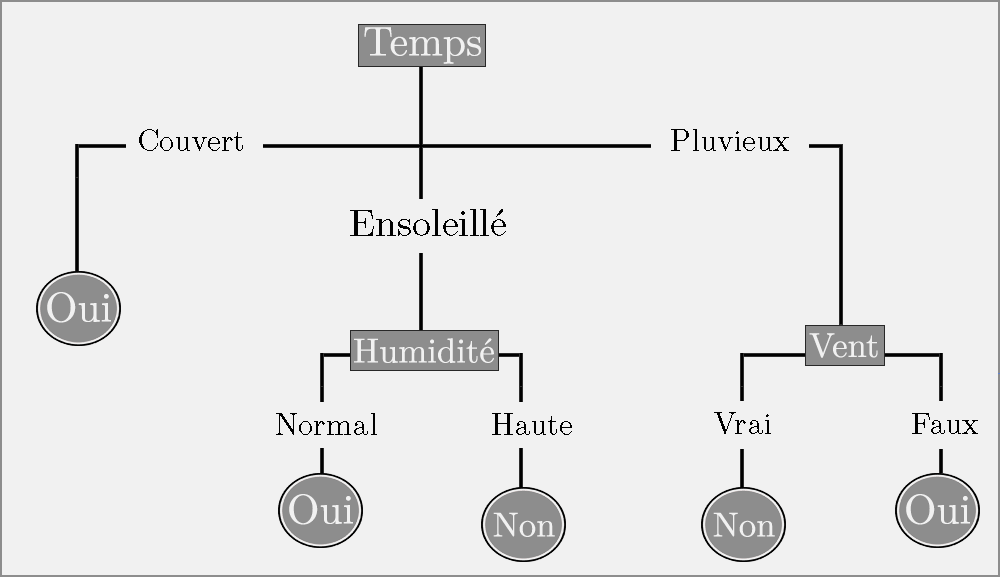
\includegraphics[scale=3]{figure_GI}
\caption{Arbre de décision construit avec ID3 en utilisant le Gain d'information}
\end{center}
\end{figure}





\chapter{\textsc{Rapport de Gain}}

\section{Definition}
Mis au point toujours par \textsc{Quinlan}, le but de ce critère est de normaliser le rapport de gain, car ce dernier a tendance a favoriser les attributs ayant beaucoup de modalités.
Prenons l'exemple d'un attribut qui a autant de modalité qu'il y a de valeur (disons N), avec la Gain d'information, cette attribut sera choisi comme attribut de division, donnant ainsi N sous arbre. Or, le but de la classification est de créer des classes d'individus, et non pas créer une classe pour chaque individu. Avec un calcule normalisé, cet attribut ne sera pas privilégié.
Le rapport de gain est utilisé dans l'algorithme C4.5, qui l'amélioration de l'algorithme ID3.
\section{Formule}
Une mesure appelé \textsc{SplitInfo} est utilisée afin de normaliser le Gain d'information, la formule est la suivante : 
\begin{center}
\begin{tabular}{| l |}
\hline
$GainRatio(p,T) = \frac{Gain(p,T)}{InfoSplit(p,T)} $\\
$SplitInfo(p,T) = - \sum_{j=1}^n P_j * log_2 (P_j)$\\

% 1-\sum\limits_{j=0}^n 1- P_j^2$\\
\hline
\end{tabular}
\end{center}

\section{Exemple}
Reprenons le même ensemble de données :
\\Remarque :\\
Rappelons que le gain d'information à deja été calculé, nous pouvons donc utiliser directement les résultats suivants  :

\begin{enumerate}
\item Gain(Temps) = 0.25 
\item Gain(Température) = 0.05 
\item Gain(Humidité) = 0.15
\item Gain(Vent) = 0.05
\end{enumerate}
\newpage
\begin{figure}[!h]
\begin{small}

\begin{center}

\caption{Ensemble de données de départ}
\begin{tabular}{| l | l | l | l | l |}
\hline
\rowcolor{gray!25}
Temps & Température & Humidité & Vent & Jouer \\
\hline
Ensoleillé & Haute & Haute & Faux & \cellcolor{green}Non \\
\hline
Ensoleillé & Haute & Haute & Vrai & \cellcolor{green}Non \\
\hline
Couvert & Haute & Haute & Faux & \cellcolor{yellow}Oui \\
\hline
Pluvieux & Basse & Haute & Faux & \cellcolor{yellow}Oui \\
\hline
Pluvieux & Moyenne & Normal & Faux & \cellcolor{yellow}Oui \\
\hline
Pluvieux & Moyenne & Normal & Vrai &  \cellcolor{green}Non \\
\hline
Couvert & Moyenne & Normal & Vrai &  \cellcolor{yellow}Oui \\
\hline
Ensoleillé & Basse & Haute & Faux &  \cellcolor{green}Non \\
\hline
Ensoleillé & Moyenne & Normal & Faux &  \cellcolor{yellow}Oui \\
\hline
Pluvieux & Basse & Normal & Faux &  \cellcolor{yellow}Oui \\
\hline
Ensoleillé & Basse & Normal & Vrai &  \cellcolor{yellow}Oui \\
\hline
Couvert & Basse & Haute & Vrai &  \cellcolor{yellow}Oui \\
\hline
Couvert & Haute & Normal & Faux &  \cellcolor{yellow}Oui \\
\hline
Pluvieux & Moyenne & Haute & Vrai &  \cellcolor{green}Non \\
\hline
\end{tabular}
\end{center}
\end{small}

\end{figure}

\begin{itemize}



\item Calcul d'InfoSplit de chaque attribut \\
\begin{itemize}
\item Temps\\
Nous avons :\\
 

\[Nombre \ de \ modalité \ : \ 3 \ \left\{ 
\begin{array}{l l}
  Ensoleillé : & \quad \text{ 5}\\
  Pluvieux : & \quad \text{ 5}\\ 
  Couvert : & \quad \text{ 4}\\
  \end{array} \right. \]
  
$InfoSplit(Temps) = - (\frac{5}{14}Log_2(\frac{5}{14}) + \frac{5}{14}Log_2(\frac{5}{14}) + \frac{4}{14}Log_2(\frac{4}{14}))\\
InfoSplit(Temps) = 1.577$

\item Température
$InfoSplit(Température) = - (\frac{5}{14}Log_2(\frac{5}{14}) + \frac{5}{14}Log_2(\frac{5}{14}) + \frac{4}{14}Log_2(\frac{4}{14}))\\
InfoSplit(Température) = 1.577$


\item Humidité
$InfoSplit(Température) = - (\frac{7}{14}Log_2(\frac{7}{14}) + \frac{7}{14}Log_2(\frac{7}{14}) \\
InfoSplit(Température) = 1$


\item Vent
$InfoSplit(Température) = - (\frac{8}{14}Log_2(\frac{8}{14}) + \frac{6}{14}Log_2(\frac{6}{14}) \\
InfoSplit(Température) = 0.98$
\end{itemize}


\item Calcul du rapport de gain de chaque attribut \\

\begin{enumerate}
\item $GainRatio(Temps) = \frac{0.25}{1.577} = 0.15 $\\ 
\item $GainRatio(Température)  = \frac{0.05}{1.577} = 0.03$  \\
\item $GainRatio(Humidité)  = \frac{0.15}{1} = 0.15$ \\
\item $GainRatio(Vent)  = \frac{0.05}{0.98} = 0.151$
\end{enumerate}

Nous remarquons que le résultat de la recherche de l'attribut de division a changé, nous pouvons donc continuer le calcul avec l'attribut Humidité, qui, avec ses deux valeurs, été désavantagé comparé à l'attribut Température (3 valeurs) lors de l'utilisation du Gain d'information.
\end{itemize}

\chapter{Chi-Square}
%((2-3.21)^2)/3.21+((3-1.78)^2)/1.78+((3-3.21)^2)/3.21+((2-1.78)^2)/1.78+((4-2.57)^2)/2.57+((0-1.43)^2)/%1.43 = 3.55

\section{Définition}
Le Chi-square est un test statistique, il permet, à partir d'un tableau de contingence, de comparer l'indépendance des variabes, afin de savoir si elles sont liées, autrement dis, il permet de vérifier si les distribution des variables différent les unes des autres.
Ce test est utilisé comme critère d'arrêt dans l'algorithme d'arbre de décision CHAID (\textsc{CHi-squared Automatic Interaction Detector)}
\section{Formule}
Le calcule du Chi-square ($X^^2$ repose sur deux tableau, ça savoir :
\begin{itemize}
\item Tableau d'observation 
\item Tableau d'estimation 
\end{itemize}

\section{Exemple}
Soit l'ensemble de données suivants :

\begin{figure}[!h]
\begin{center}

\caption{Ensemble de données de départ}
\begin{tabular}{| l | l | l | l | l |}
\hline
\rowcolor{gray!25}
Temps & Température & Humidité & Vent & Jouer \\
\hline
Ensoleillé & Haute & Haute & Faux & \cellcolor{green}Non \\
\hline
Ensoleillé & Haute & Haute & Vrai & \cellcolor{green}Non \\
\hline
Couvert & Haute & Haute & Faux & \cellcolor{yellow}Oui \\
\hline
Pluvieux & Basse & Haute & Faux & \cellcolor{yellow}Oui \\
\hline
Pluvieux & Moyenne & Normal & Faux & \cellcolor{yellow}Oui \\
\hline
Pluvieux & Moyenne & Normal & Vrai &  \cellcolor{green}Non \\
\hline
Couvert & Moyenne & Normal & Vrai &  \cellcolor{yellow}Oui \\
\hline
Ensoleillé & Basse & Haute & Faux &  \cellcolor{green}Non \\
\hline
Ensoleillé & Moyenne & Normal & Faux &  \cellcolor{yellow}Oui \\
\hline
Pluvieux & Basse & Normal & Faux &  \cellcolor{yellow}Oui \\
\hline
Ensoleillé & Basse & Normal & Vrai &  \cellcolor{yellow}Oui \\
\hline
Couvert & Basse & Haute & Vrai &  \cellcolor{yellow}Oui \\
\hline
Couvert & Haute & Normal & Faux &  \cellcolor{yellow}Oui \\
\hline
Pluvieux & Moyenne & Haute & Vrai &  \cellcolor{green}Non \\
\hline
\end{tabular}
\end{center}

\end{figure}
\newpage
\begin{itemize}
\item Calcul du Ch-square $(X^2)$ de chaque attribut
\begin{enumerate}
\item Temps

\begin{table}[!h]
\begin{small}
\begin{tabular}{cc}

    \begin{minipage}{.5\linewidth}
   
\begin{tabular}{| l | l | l | l | l |}
\hline
 & Oui & Non & Total\\
\hline
Ensoleillé & 2 & 3 & 5\\
\hline
Pluvieux & 3 & 2 & 5 \\
\hline
Couvert & 4 & 0 & 4 \\
\hline
Total & 9 & 5 & 14 \\
\hline
\end{tabular} 
      \caption{Tableau d'observation}

    \end{minipage} &

    \begin{minipage}{.5\linewidth}
\begin{tabular}{| l | l | l |}
\hline
 & Oui & Non\\
\hline
Ensoleillé & $\frac{5*9}{14} = 3.21$ & $\frac{5*5}{14} = 1.78$\\
\hline
Pluvieux & $\frac{5*9}{14} = 3.21$ & $\frac{5*5}{14} = 1.78$ \\
\hline
Couvert & $\frac{4*9}{14} = 2.57$ & $\frac{4*5}{14} = 1.43$  \\
\hline
\end{tabular} 
      \caption{Tableau d'estimation}
 
    \end{minipage} 
\end{tabular}
\end{small}
\end{table}


$X^2(Temps) = \frac{(2-3.21)^2}{3.21}+\frac{(3-1.78)^2}{1.78}+\frac{(3-3.21)^2}{3.21}+\frac{(2-1.78)^2}{1.78}+\frac{(4-2.57)^2}{2.57}+\frac{(0-1.43)^2}{1.43}\\
X^2(Temps) = 3.55$


\item Température

\begin{table}[!h]
\begin{small}
\begin{tabular}{cc}

    \begin{minipage}{.5\linewidth}
   
\begin{tabular}{| l | l | l | l | l |}
\hline
 & Oui & Non & Total\\
\hline
Haute & 2 & 2 & 4\\
\hline
Basse & 4 & 1 & 5 \\
\hline
Moyenne & 3 & 2 & 5 \\
\hline
Total & 9 & 5 & 14 \\
\hline
\end{tabular} 
      \caption{Tableau d'observation}

    \end{minipage} &

    \begin{minipage}{.5\linewidth}
\begin{tabular}{| l | l | l |}
\hline
 & Oui & Non\\
\hline
Haute & $\frac{4*9}{14} = 2.57$ & $\frac{4*5}{14} = 1.43$\\
\hline
Basse & $\frac{5*9}{14} = 3.21$ & $\frac{5*5}{14} = 1.78$ \\
\hline
Moyenne & $\frac{5*9}{14} = 3.21$ & $\frac{5*5}{14} = 1.78$  \\
\hline
\end{tabular} 
      \caption{Tableau d'estimation}
 
    \end{minipage} 
\end{tabular}
\end{small}
\end{table}

$X^2(Température) = \frac{(2-2.57)^2}{2.57}+\frac{(2-1.43)^2}{1.43}+\frac{(4-3.21)^2}{3.21}+\frac{(2-1.78)^2}{1.78}+\frac{(3-3.21)^2}{3.21}+\frac{(2-1.78)^2}{1.78}\\
X^2(Température) = 0.62$

\item Humidité

\begin{table}[!h]
\begin{small}
\begin{tabular}{cc}

    \begin{minipage}{.5\linewidth}
   
\begin{tabular}{| l | l | l | l | l |}
\hline
 & Oui & Non & Total\\
\hline
Haute & 3 & 4 & 7\\
\hline
Normal & 6 & 1 & 7 \\
\hline
Total & 9 & 5 & 14 \\
\hline
\end{tabular} 
      \caption{Tableau d'observation}

    \end{minipage} &

    \begin{minipage}{.5\linewidth}
\begin{tabular}{| l | l | l |}
\hline
 & Oui & Non\\
\hline
Haute & $\frac{7*9}{14} = 4.5$ & $\frac{7*5}{14} = 2.5$\\
\hline
Basse & $\frac{7*9}{14} = 4.5$ & $\frac{7*5}{14} = 2.5$ \\
\hline
\end{tabular} 
      \caption{Tableau d'estimation}
 
    \end{minipage} 
\end{tabular}
\end{small}
\end{table}

$X^2(Humidité) = \frac{(3-4.5)^2}{4.5}+\frac{(4-2.5)^2}{2.5}+\frac{(6-4.5)^2}{4.5}+\frac{(1-2.5)^2}{2.5}\\
X^2(Humidité) = 2.8$

\item Vent

\begin{table}[!h]
\begin{small}
\begin{tabular}{cc}

    \begin{minipage}{.5\linewidth}
   
\begin{tabular}{| l | l | l | l | l |}
\hline
 & Oui & Non & Total\\
\hline
Vrai & 3 & 3 & 6\\
\hline
Faux & 6 & 2 & 8 \\
\hline
Total & 9 & 5 & 14 \\
\hline
\end{tabular} 
      \caption{Tableau d'observation}

    \end{minipage} &

    \begin{minipage}{.5\linewidth}
\begin{tabular}{| l | l | l |}
\hline
 & Oui & Non\\
\hline
Haute & $\frac{6*9}{14} = 3.86$ & $\frac{6*5}{14} = 2.14$\\
\hline
Basse & $\frac{8*9}{14} = 5.14$ & $\frac{8*5}{14} = 2.86$ \\
\hline
\end{tabular} 
      \caption{Tableau d'estimation}
 
    \end{minipage} 
\end{tabular}
\end{small}
\end{table}

$X^2(Humidité) = \frac{(3-3.86)^2}{3.86}+\frac{(3-2.14)^2}{2.14}+\frac{(6-5.14)^2}{5.14}+\frac{(2-2.86)^2}{2.86}\\
X^2(Temps) = 0.94$

\end{enumerate}
La division se fera par rapport à l'attribut Temps (celui ayant la plus grande valeur $X^2$
\newpage
\item Division

\begin{figure}[!h]
\begin{center}

\begin{tabular}{| l | l | l | l | l |}
\hline
\rowcolor{gray!25}
Temps & Température & Humidité & Vent & Jouer \\
Couvert & Haute & Haute & Faux & \cellcolor{yellow}Oui \\
Couvert & Moyenne & Normal & Vrai &  \cellcolor{yellow}Oui \\
Couvert & Basse & Haute & Vrai &  \cellcolor{yellow}Oui \\
\hline
Couvert & Haute & Normal & Faux &  \cellcolor{yellow}Oui \\
\hline
\end{tabular}
\end{center}
\end{figure}


\begin{figure}[!h]
\begin{center}

\caption{Sous ensemble A}

\end{center}
Sous ensemble homogène par rapport à la variable de classes, arrêt.
\end{figure}

\begin{table}[!h]
\begin{small}
\begin{tabular}{cc}

    \begin{minipage}{.5\linewidth}
   
\begin{tabular}{| l | l | l | l | l |}
\hline
Temps & Température & Humidité & Vent & Jouer \\
\hline
Pluvieux & Basse & Haute & Faux & \cellcolor{yellow}Oui \\
\hline
Pluvieux & Moyenne & Normal & Faux & \cellcolor{yellow}Oui \\
\hline
Pluvieux & Moyenne & Normal & Vrai &  \cellcolor{green}Non \\
\hline
Pluvieux & Basse & Normal & Faux &  \cellcolor{yellow}Oui \\
\hline
Pluvieux & Moyenne & Haute & Vrai &  \cellcolor{green}Non \\
\hline
\end{tabular} 
\caption{Sous ensemble B}

    \end{minipage} &

    \begin{minipage}{.5\linewidth}
\begin{tabular}{| l | l | l | l | l |}
\hline
Temps & Température & Humidité & Vent & Jouer \\
\hline
Ensoleillé & Haute & Haute & Faux & \cellcolor{green}Non \\
\hline
Ensoleillé & Haute & Haute & Vrai & \cellcolor{green}Non \\
\hline
Ensoleillé & Basse & Haute & Faux &  \cellcolor{green}Non \\
\hline
Ensoleillé & Moyenne & Normal & Faux &  \cellcolor{yellow}Oui \\
\hline
Ensoleillé & Basse & Normal & Vrai &  \cellcolor{yellow}Oui \\
\hline
\end{tabular} 
\caption{Sous ensemble C}
 
    \end{minipage} 
\end{tabular}
\end{small}
\end{table}

\item Développement du sous ensemble B
\begin{enumerate}
\item Température 

\begin{table}[!h]
\begin{small}
\begin{tabular}{cc}

    \begin{minipage}{.5\linewidth}
   
\begin{tabular}{| l | l | l | l | l |}
\hline
 & Oui & Non & Total\\
\hline
Moyenne & 1 & 2 & 3\\
\hline
Basse & 2 & 0 & 2 \\
\hline
Total & 3 & 2 & 5 \\
\hline
\end{tabular} 
      \caption{Tableau d'observation}

    \end{minipage} &

    \begin{minipage}{.5\linewidth}
\begin{tabular}{| l | l | l |}
\hline
 & Oui & Non\\
\hline
Haute & $\frac{3*3}{5} = 1.8$ & $\frac{3*2}{5} = 1.2$\\
\hline
Basse & $\frac{2*3}{5} = 1.2$ & $\frac{2*2}{5} = 0.8$ \\
\hline
\end{tabular} 
      \caption{Tableau d'estimation}
 
   \end{minipage} 
\end{tabular}
\end{small}
\end{table}

$X^2(Température) = \frac{(1-1.8)^2}{1.8}+\frac{(2-1.2)^2}{1.2}+\frac{(2-1.2)^2}{1.2}+\frac{(0-0.8)^2}{0.8}\\
X^2(Température) = 2.22$





\item Humidité


\begin{table}[!h]
\begin{small}
\begin{tabular}{cc}

    \begin{minipage}{.5\linewidth}
   
\begin{tabular}{| l | l | l | l | l |}
\hline
 & Oui & Non & Total\\
\hline
Haute & 1 & 1 & 2\\
\hline
Normal & 2 & 1 & 3 \\
\hline
Total & 3 & 2 & 5 \\
\hline
\end{tabular} 
      \caption{Tableau d'observation}

    \end{minipage} &

    \begin{minipage}{.5\linewidth}
\begin{tabular}{| l | l | l |}
\hline
 & Oui & Non\\
\hline
Haute & $\frac{2*3}{5} = 1.2$ & $\frac{2*2}{5} = 0.8$\\
\hline
Basse & $\frac{3*3}{5} = 1.8$ & $\frac{3*2}{5} = 1.2$ \\
\hline
\end{tabular} 
      \caption{Tableau d'estimation}
 
   \end{minipage} 
\end{tabular}
\end{small}
\end{table}

$X^2(Humidité) = \frac{(1-1.2)^2}{1.2}+\frac{(1-0.8)^2}{0.8}+\frac{(2-1.8)^2}{1.8}+\frac{(1-1.2)^2}{1.2}\\
X^2(Humidité) = 0.13$



\item Vent

\begin{table}[!h]
\begin{small}
\begin{tabular}{cc}

    \begin{minipage}{.5\linewidth}
   
\begin{tabular}{| l | l | l | l | l |}
\hline
 & Oui & Non & Total\\
\hline
Vrai & 0 & 2 & 2\\
\hline
Faux & 3 & 0 & 3 \\
\hline
Total & 3 & 2 & 5 \\
\hline
\end{tabular} 
      \caption{Tableau d'observation}

    \end{minipage} &

    \begin{minipage}{.5\linewidth}
\begin{tabular}{| l | l | l |}
\hline
 & Oui & Non\\
\hline
Haute & $\frac{2*3}{5} = 1.2$ & $\frac{2*2}{5} = 0.8$\\
\hline
Basse & $\frac{3*3}{5} = 1.8$ & $\frac{3*2}{5} = 1.2$ \\
\hline
\end{tabular} 
      \caption{Tableau d'estimation}
 
   \end{minipage} 
\end{tabular}
\end{small}
\end{table}

$X^2(Vent) = \frac{(0-1.2)^2}{1.2}+\frac{(2-0.8)^2}{0.8}+\frac{(3-1.8)^2}{1.8}+\frac{(0-1.2)^2}{1.2}\\
X^2(Vent) = 5$
\end{enumerate}
Le sous ensemble B sera donc divisé par rapport a l'attribut Vent.



\begin{table}[!h]
\begin{small}
\begin{tabular}{cc}

    \begin{minipage}{.5\linewidth}
   
\begin{tabular}{| l | l | l | l | l |}
\hline
Temps & Température & Humidité & Vent & Jouer \\
\hline
Pluvieux & Moyenne & Normal & Vrai &  \cellcolor{green}Non \\
\hline
Pluvieux & Moyenne & Haute & Vrai &  \cellcolor{green}Non \\
\hline
\end{tabular}
      \caption{Sous ensemble D}

    \end{minipage} &

    \begin{minipage}{.5\linewidth}
\begin{tabular}{| l | l | l | l | l |}
\hline
Temps & Température & Humidité & Vent & Jouer \\
\hline
Pluvieux & Basse & Haute & Faux & \cellcolor{yellow}Oui \\
\hline
Pluvieux & Moyenne & Normal & Faux & \cellcolor{yellow}Oui \\
\hline
Pluvieux & Basse & Normal & Faux &  \cellcolor{yellow}Oui \\
\hline
\end{tabular}

      \caption{Sous ensemble E}
 
   \end{minipage} 
\end{tabular}
\end{small}	
Les deux sous ensemble C et D sont homogène par rapport a la variable de classe, arrêt.
\end{table}
Développement du sous ensemble C. Faire exactement le même calcul, et l'attribut ayant la plus grande valeur de $X^2$ sera l'attribut Humidité. Ce qui donnera les deux sous ensemble suivant :

\begin{table}[!h]
\begin{small}
\begin{tabular}{cc}

    \begin{minipage}{.5\linewidth}
   
\begin{tabular}{| l | l | l | l | l |}
\hline
Temps & Température & Humidité & Vent & Jouer \\
\hline
Ensoleillé & Moyenne & Normal & Faux &  \cellcolor{yellow}Oui \\
\hline
Ensoleillé & Basse & Normal & Vrai &  \cellcolor{yellow}Oui \\
\hline
\end{tabular}

      \caption{Sous ensemble F}

    \end{minipage} &

    \begin{minipage}{.5\linewidth}


\begin{tabular}{| l | l | l | l | l |}
\hline
Temps & Température & Humidité & Vent & Jouer \\
\hline
Ensoleillé & Haute & Haute & Faux & \cellcolor{green}Non \\
\hline
Ensoleillé & Haute & Haute & Vrai & \cellcolor{green}Non \\
Ensoleillé & Basse & Haute & Faux &  \cellcolor{green}Non \\
\hline
\end{tabular}
      \caption{Sous ensemble G}
 
   \end{minipage} 
\end{tabular}
\end{small}	
Les deux sous ensemble D et E sont homogène par rapport a la variable de classe, arrêt.
\end{table}
\end{itemize}
TOUS LES SOUS ENSEMBLE SONS HOMOGÈNES : CRITÈRE D'ARRÊT ATTEINT.

\begin{figure}[!h]
\begin{center}
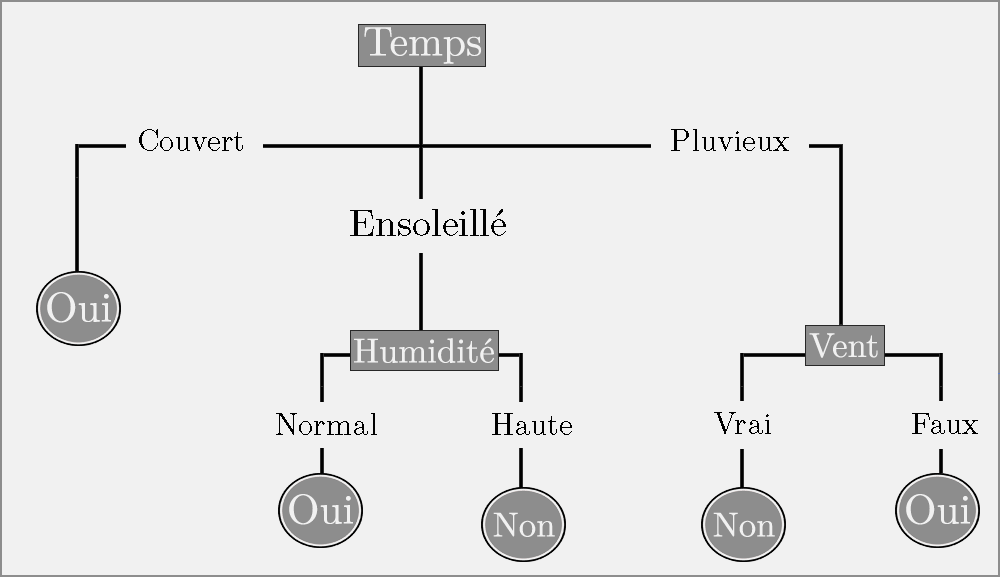
\includegraphics[scale=3]{figure_GI}
\caption{Arbre de décision construit avec ID3 en utilisant le Gain d'information}
\end{center}
\end{figure}

\end{document}

